%!TEX root = ../dissertation.tex
%\begin{savequote}[75mm]
%Nulla facilisi. In vel sem. Morbi id urna in diam dignissim feugiat. Proin molestie tortor eu velit. Aliquam erat volutpat. Nullam ultrices, diam tempus vulputate egestas, eros pede varius leo.
%\qauthor{Quoteauthor Lastname}
%\end{savequote}

\chapter{Experiments}

Summarizing the work done until now, it has been created a sentiment analysis dataset based on italian automotive forums by crawling web resources and then scraping HTML pages. Then, the dataset has been labeled by many workers, obtaining a sufficiently large amount of data to be processed. The next phase consisted in defining some machine learning models in order to make both topic detection and sentiment classification. In this Chapter, will be firstly presented, as a benchmark, results obtained running the models on a Twitter's dataset, and then the results obtained on the created dataset.\\
Every test will be presented with a common framework: 
\begin{itemize}
	\item Results obtained with a classification before features selection;
	\item Features selection and most important features;
	\item Results obtained after features selection;
\end{itemize}
Classification results will be presented both visually using confusion matrices and using numerical scores.\\
Since used algorithms don't require huge amount of computational power, runs have been made on a 2019 consumer technology with the following specifics:
% CPU, RAM,
\begin{center}
	\begin{tabular}{ |c||c| } 
		\hline
		\textbf{CPU} & Intel(R) Core(TM) i7-8550U CPU @ 1.80GHz 4 cores, 8 threads\\ 
		\hline
		\textbf{RAM} & 16GB DDR4 \\
		\hline
		\textbf{O.S.} & Ubuntu 18.04 \\
		\hline
	\end{tabular}
\end{center}
Where it has been installed a Python 3.7 release on a Jupyter Notebook.


\section{Experiments on Twitter's Airline Dataset}

The first series of experiments concerns the Twitter's Airline dataset described in Section 2.1.6. The purpose of these tests is to verify the goodness of the models in a dataset that is plenty of well labeled comments. The reference result on tweets sentiment classification can be extracted from \cite{Zimbra:2018:STS:3210372.3185045}, where BPEF algorithm reached the best results with an average accuracy of 71.38\% on sentiment classification on five different datasets, but average performance of all models stay around 65\%, so a similar result will be positive.\\
The dataset consists in 14640 labeled tweets, divided into 3099 positives, 2363 neutrals and 9178 negatives. Due to the plenty of data, all classes were balanced, with the number of comments of the minority class. Successively, the dataset were divided into training set and test set, respectively the 80\% and the 20\%. Moreover, the training set were further divided into actual training set and validation set, again respectively the 80\% and the 20\%. The distribution of the datasets is:

\begin{center}
	\begin{tabular}{ | c  c  c  c | c | } 
		\hline
		& \textbf{Positives} & \textbf{Nautrals} & \textbf{Negatives} & \textbf{Total} \\
		\hline
		\textbf{Training} & 960 & 960 & 960 & 2880 \\ 
		\hline
		\textbf{Validation} & 240 & 240 & 240 & 720 \\ 
		\hline
		% TODO riempi test e fai classificazione
		\textcolor{red}{TEST}
		\textbf{Test} &  &  & &\\
		\hline
		%\label{table:twitt-class-data}
		%\caption{Class distribution of training, validation and test sets of tweets' sentiment classification.}
	\end{tabular}
\end{center}

Due to the class balance, also accuracy score is meaningful, so it is presented along with F1-macro and F1-micro scores.


\subsection{Sentiment Classification with SVM}

After preprocessing and vectorization with TF-IDF method on the training set, involving both unigrams and bigrams, the outcome dimension counts 22.486 features. Data are stored in a sparse matrix 2880x22.486 with 50.006 stored elements, so as expected, it is actually very sparse.\\
A first model train is performed involving all features, optimizing the regularization parameter $C$ from 7 candidates exponentially equally spaced from $10^{-3}$ to $10^3$, searching for the best F1-macro score.\\
The selected model is the one with $C$=1, and the classification results obtained with the validation set are:

% SVM no fs
\begin{figure}[ht]
	\centering
	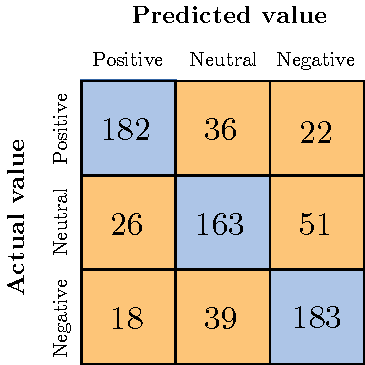
\includegraphics[scale=1]{figures/conf_matrices/twitter_snt_svm/twitter_snt_svm_bfs.pdf}
	\label{fig:tw_snt_svm_bfs}
\end{figure}

\begin{center}
	\begin{tabular}{ | c | c | } 
		\hline
		\textbf{F1-macro} & 0.734 \\
		\hline
		\textbf{F1-micro} & 0.733 \\ 
		\hline
		\textbf{Accuracy} & 0.734 \\ 
		\hline
	\end{tabular}
\end{center}

It is possible to see that the baseline method without feature selection reaches good results, aligned with state of the art. From the confusion matrix, diagonal values (which are the correctly classified) are in fact the majority, and also the accuracy of 70,4\% reflects the visual considerations.\\
The sorted weights of the three binary classifiers that constitute the one-versus-one multiclass classifier are shown in Figure \ref{fig:svm-fs}.

% fs

\begin{figure}[H]
	\centering
	\begin{subfigure}{1\textwidth} % width of left subfigure
		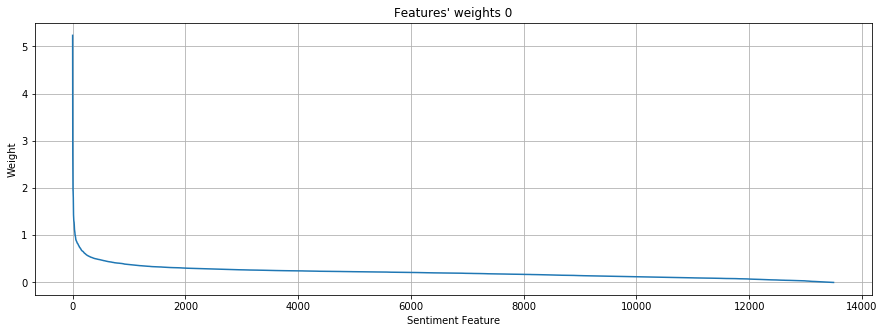
\includegraphics[width=\textwidth]{figures/conf_matrices/twitter_snt_svm/svm_fs_1.png}
	\end{subfigure}
	\begin{subfigure}{1\textwidth} % width of right subfigure
		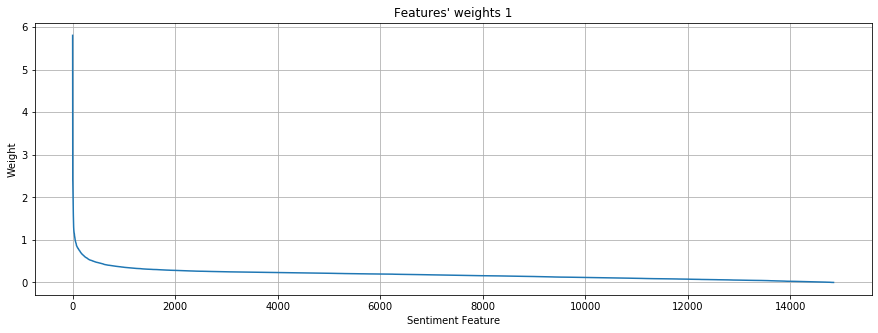
\includegraphics[width=\textwidth]{figures/conf_matrices/twitter_snt_svm/svm_fs_2.png}
	\end{subfigure}
	\begin{subfigure}{1\textwidth} % width of right subfigure
		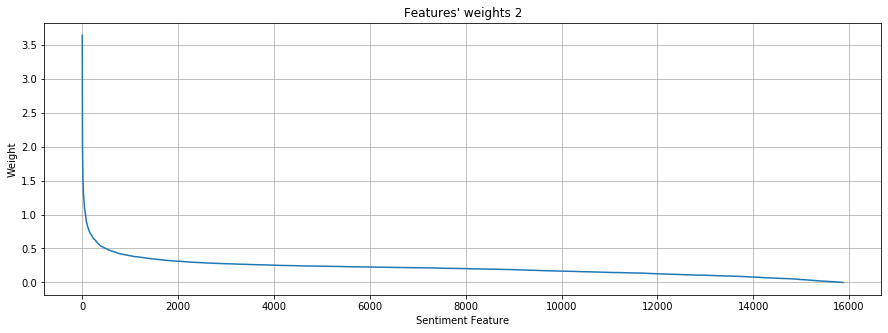
\includegraphics[width=\textwidth]{figures/conf_matrices/twitter_snt_svm/svm_fs_3.png}
	\end{subfigure}
	\caption{Features' weights of the three binary classifiers of the one-versus-one multiclass classifier} % caption for whole figure
	\label{fig:svm-fs}
\end{figure}

After some manual tries, the selected cutoff values are respectively 0.3, 0.3 and 0.2, obtaining 9564 final selected features, where most important with respect every binary classifier are shown in Figure % TODO features piu importanti svm
\textcolor{red}{FEATURE PIU IMPORTANTI}
% SVM fs
 Retraining the model using just selected features, the results on the validation set are:
% TODO sistemare
\begin{figure}[H]
	\centering
	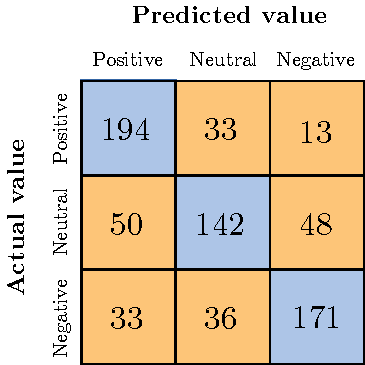
\includegraphics[scale=1]{figures/conf_matrices/twitter_snt_svm/twitter_snt_svm_afs.pdf}
	\label{fig:tw_snt_svm_afs}
\end{figure}

\begin{center}
	\begin{tabular}{ | c | c | } 
		\hline
		\textbf{F1-macro} & 0.702 \\
		\hline
		\textbf{F1-micro} & 0.704 \\ 
		\hline
		\textbf{Accuracy} & 0.704 \\ 
		\hline
	\end{tabular}
\end{center}

After feature selection it is possible to notice a loss of performance due to the removal of some relevant features. However, features selection has the goal to make the model more stable, rather that more performing. The final metrics still highlight performance close to state of the art models, and looking at the result on test data, .... % TODO test classfication

\textcolor{red}{TEST CLASSIFICATION}


\subsection{Sentiment Classification with Revised BPEF}

At this point the goal is to enhance the previous model with the revised BPEF ensemble. In this model, feature's relevance is calculated using the information gain metric, and since it is based on dataset's distribution instead of model's weights, it is possible to calculate it as the first phase, for every combination of the model's features parameters.\\
The outcome of features ranking is very similar for all features parameters and has the following trend:

\begin{figure}[ht]
	\centering
	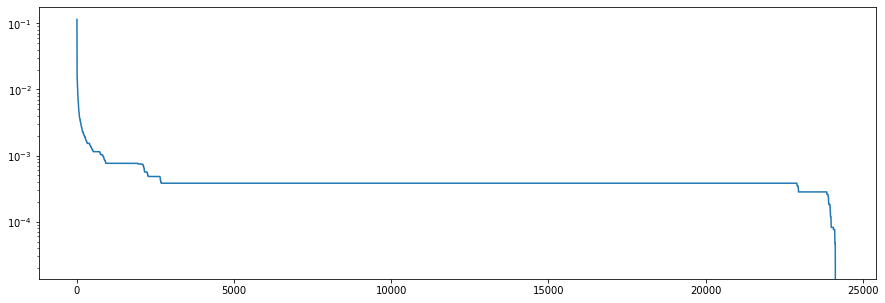
\includegraphics[width=\textwidth]{figures/conf_matrices/twitter_snt_bpef/bpef_fs_1.png}
	\label{fig:twitter_bpef_fs_1}
\end{figure}

It is possible to notice that there are just few features with higher information gain, while most have a flat trend. The strategy for features selection was to set the cutoff value in correspondence of the starting of the flat curve, in order to keep just features with higher information gain.\\
Before features selection it were counted the following number of features:

\begin{center}
	\begin{tabular}{ c  c  c } 
		\hline
		\textbf{Feature name} & \textbf{Word summarizing} & \textbf{\# Features} \\
		\hline
		word & false & 24.206 \\ 
		\hline
		word & true & 22.485 \\ 
		\hline
		pos & false & 30.282 \\ 
		\hline
		pos & true & 28.318 \\ 
		\hline
		swnt & false & 22.789 \\ 
		\hline
		swnt & true & 21.113 \\ 
		\hline
	\end{tabular}
\end{center}

Recalling that the involved algorithms are SVM, Logistic Regression, Ra{\"i}ve Bayes and Random Forest, they are all trained optimizing with a grid search on the followings parameters:
\begin{itemize}
	\item SVM: $C$ from $10^{-3}$ to $10^3$ with 7 exponentially evenly spaced values;
	\item Logistic Regression: $C$ from $10^{-3}$ to $10^3$ with 7 exponentially evenly spaced values;
	\item Random Forest: 
	\begin{itemize}
		\item Number of estimators: [201, 501]
		\item Maximum of looked features on split: [auto, $log_2$]
		\item Maximum depth of the tree: [10, 100]
		\item Split criterion: [gini, entropy]
	\end{itemize}
\end{itemize}

% BPEF no fs
The classification without features selection on validation data gives the following results:

% TODO bpef twitter nofs conf matrix

\begin{figure}[H]
	\centering
	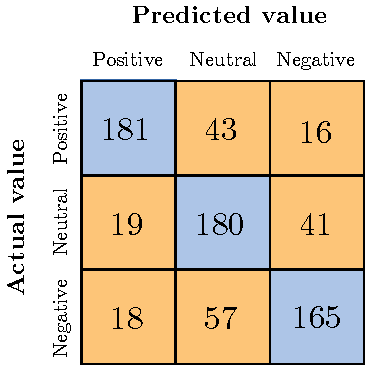
\includegraphics[scale=1]{figures/conf_matrices/twitter_snt_bpef/twitter_snt_bpef_bfs.pdf}
	\label{fig:tw_snt_bpef_bfs}
\end{figure}

\begin{center}
	\begin{tabular}{ | c | c | } 
		\hline
		\textbf{F1-macro} & 0.732 \\
		\hline
		\textbf{F1-micro} & 0.731 \\ 
		\hline
		\textbf{Accuracy} & 0.731 \\ 
		\hline
	\end{tabular}
\end{center}

% fs

The results are very similar to the ones reached with SVM classificator without features selection. Setting a cutoff value for feature selection equal to $4\times10^{-4}$, the number of selected features becomes:

\begin{center}
	\begin{tabular}{ c  c  c } 
		\hline
		\textbf{Feature name} & \textbf{Word summarizing} & \textbf{\# Features} \\
		\hline
		word & false & 2.665 \\ 
		\hline
		word & true & 2.622 \\ 
		\hline
		pos & false & 3.181 \\ 
		\hline
		pos & true & 3.057 \\ 
		\hline
		swnt & false & 2.657 \\ 
		\hline
		swnt & true & 2.612 \\ 
		\hline
	\end{tabular}
\end{center}

% BPEF fs

Which are less than one third than the previously case. Training again the model optimizing the same hyperparameters with the same grid search, the obtained results are the followings:

\begin{figure}[H]
	\centering
	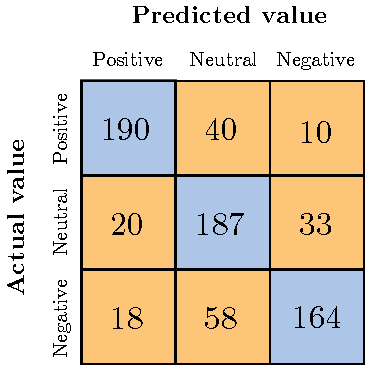
\includegraphics[scale=1]{figures/conf_matrices/twitter_snt_bpef/twitter_snt_bpef_afs.pdf}
	\label{fig:tw_snt_bpef_afs}
\end{figure}

\begin{center}
	\begin{tabular}{ | c | c | } 
		\hline
		\textbf{F1-macro} & 0.753 \\
		\hline
		\textbf{F1-micro} & 0.751 \\ 
		\hline
		\textbf{Accuracy} & 0.751 \\ 
		\hline
	\end{tabular}
\end{center}

Looking at the scores, it is easy to notice the better performance of the BPEF revisitation against the SVM model, even considering very less features. Moreover, due to the strong cut of the features and the optimal results, it is possible to suppose that the feature selection method returns an actual set of relevant features, that combined with the stability of the ensemble lead to prefer this model against the previous one. These considerations are confirmed looking at the results on the test set:

% TODO risultati test set
\textcolor{red}{RISULTATI TEST SET}


\section{Experiments on Italian's Automotive Dataset}

Now that some results are available, it is possible to state the effectiveness of the implemented algorithms. In this section the same models for sentiment analysis will be executed on the Italian automotive dataset. Moreover, have been designed models for relevance detection that will be implemented for the cascade classifier. For all classification have been involved "Text" and "Quote" columns of the dataset, in the way that was mentioned in the previous chapter: both techniques for texts combinations were tested, and similar but better results were obtained without adding the suffix that subdivides text's words against quote's words. \\

\subsubsection{Relevance Detection}

Before sentiment classification, it has been studied the task of relevance detection, where the goal consists on identifying weather a comment talks about a given topic. In the dataset, relevance is identified in the presence of a sentiment expression, whether it is "positive", "negative" or "neutral", while the irrelevance is obviously identified in the "irrelevant" label. The problem is then summarized in a binary text classification problem, that will constitute the first block of the cascade classificator.\\
Relevance is studied one topic at time, in fact the whole study of the models was made on the class "Engine", and then exported for all others. For the class "Engine" the dataset is constituted of 7183 comments, 866 of which are classified as "relevant", so as said, unbalance is really visible. The dataset is splitted into training data and test data, respectively the 80\% and 20\%. Then, the training dataset has been further splitted into actual training and validation sets, respectively the 80\% and 20\%. The distribution of the datasets is:

\begin{center}
	\begin{tabular}{ | c  c  c | c | } 
		\hline
		& \textbf{Relevant} & \textbf{Irrelevant} & \textbf{Total} \\
		\hline
		% TODO riempi training
		
		\textbf{Training} \textcolor{red}{TRAINING} &  &  &  \\ 
		\hline
		\textbf{Validation} & 133 & 1017 & 1150 \\ 
		\hline
		% TODO riempi test e fai classificazione
		\textbf{Test} \textcolor{red}{TEST} &  &  & \\
		\hline
		%\label{table:twitt-class-data}
		%\caption{Class distribution of training, validation and test sets of tweets' sentiment classification.}
	\end{tabular}
\end{center}

Training of the models has been made again optimizing the hyperparameters with a grid search, maximizing the F1-macro score, which is more informative for this imbalance case, in fact small changes on minority class classification give appreciable differences on the macro score, while considering the micro score, the final output is predominated by the values of the majority class. However, for comparison, if two models obtain similar F1-macro scores, the better choice falls on the one which gives the best recall, which means that it classifies less false negative samples.



\subsubsection{Sentiment Classification}

Sentiment classification involves the same techniques used for the same task with the Twitter's Airline dataset presented in the preceding section. Even for sentiment classification the algorithms were tested on the "Engine" class, but just considering the relevant comments. For this reason the dataset became similar to an usual sentiment analysis's dataset. It contains 830 total comments, divided into 317 positives, 358 neutrals and 155 negatives. Also for this phase, the dataset has been divided into training set and test set, respectively the 80\% and 20\%, and training set has been splitted into actual training set and validation set, again respectively the 80\% and 20\%. The distribution of the datasets is:

\begin{center}
	\begin{tabular}{ | c  c  c c | c | } 
		\hline
		& \textbf{Positives} & \textbf{Neutrals} & \textbf{Negatives} & \textbf{Total} \\
		\hline
		% TODO riempi training
		
		\textbf{Training} \textcolor{red}{TRAINING} &  &  &  & \\ 
		\hline
		\textbf{Validation} &  &  &  & \\ 
		\hline
		% TODO riempi test e fai classificazione
		\textbf{Test} \textcolor{red}{TEST} &  &  &  & \\
		\hline
		%\label{table:twitt-class-data}
		%\caption{Class distribution of training, validation and test sets of tweets' sentiment classification.}
	\end{tabular}
\end{center}

Since classes are largely unbalanced, undersampling the dataset for train the classifier on balanced data may lead to underfitting, so the difficulty is to control the bias due to the presence of the large "irrelevant" class.



\subsection{Relevance Detection with SVM}

% SVM no fs
The whole dataset is preprocessed involving words summarizing and vectorization with TF-IDF method for unigrams and bigrams. The outcome's dimension count 156.369 features. The number of features is a lot larger than the one seen for twitter's dataset, even in obtained with the same method. This is a consequence of the scarcity of words and expressions on Twitter's comments, and the opposite on Forums, where texts usually are more articulated. Since the number of features is very large, and the data are just few hundreds, the features selection technique may be essential for improve the stability picking just the features that are actually useful for the classification. All trainings have been made optimizing the parameter $C$ with a grid search on the values from $10^{-3}$ to $10^3$ with 7 exponentially evenly spaced values. A first training considering all features gives the following results:

\begin{figure}[H]
	\centering
	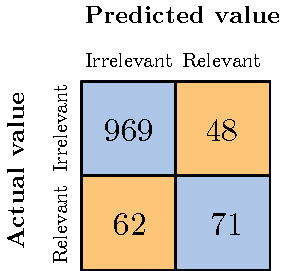
\includegraphics[scale=1]{figures/conf_matrices/ita_rel_svm/ita_rel_svm_bfs.pdf}
	\label{fig:ita_rel_svm_bfs}
\end{figure}

\begin{center}
	\begin{tabular}{ | c | c | } 
		\hline
		\textbf{F1-macro} & 0.563 \\
		\hline
		\textbf{Recall} & 0.534 \\ 
		\hline
		\textbf{Precision} & 0.597 \\ 
		\hline
	\end{tabular}
\end{center}

% fs
% TODO sistema reference
The best classifier, obtained with $C$=1000, gives the weights shown in Figure \ref{fig:ita_rel_svm_fs}, that follow the usual trend.

\begin{figure}[H]
	\centering
	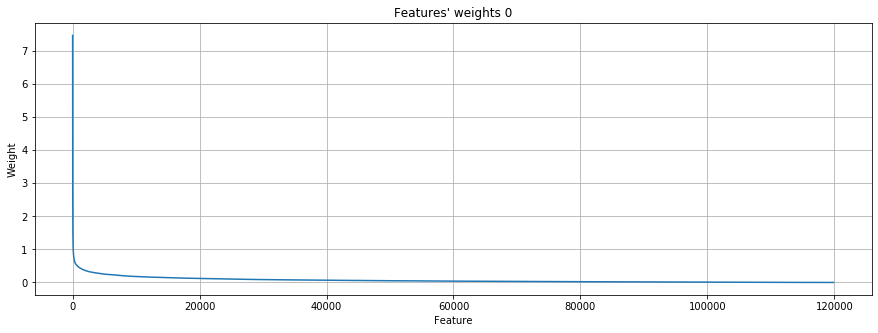
\includegraphics[width=\textwidth]{figures/conf_matrices/ita_rel_svm/ita_rel_svm_fs.png}
	\caption{Features' weights of SVM classifier for relevance detection before features selection}
	\label{fig:ita_rel_svm_fs}
\end{figure}

The cutoff value for features selection has been set to 0.2, reducing the final features' dimension to 8234. Training again the classifier on selected features, it reaches the following results:

% SVM fs

\begin{figure}[H]
	\centering
	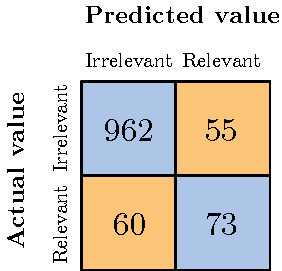
\includegraphics[scale=1]{figures/conf_matrices/ita_rel_svm/ita_rel_svm_afs.pdf}
	\label{fig:ita_rel_svm_afs}
\end{figure}

\begin{center}
	\begin{tabular}{ | c | c | } 
		\hline
		\textbf{F1-macro} & 0.559 \\
		\hline
		\textbf{Recall} & 0.549 \\ 
		\hline
		\textbf{Precision} & 0.570 \\ 
		\hline
	\end{tabular}
\end{center}

% TODO most important features
\textcolor{red}{MOST IMPORTANT FEATURES}

The final model was the one with the parameter $C$=100. Just few considerations about the previous results: Even if the task is different from the Twitter sentiment analysis, the many more difficulties are reflected in the final results, in fact performances are significantly lower. After features selection the F1-macro score obtained slightly poorer results, but the recall's improvement and the supposed improved stability makes the second model a bit better.\\
In the following paragraph, the SVM relevance detection classifier will be compared to a Logistic Regression model with the same final purpose.


\subsection{Relevance Detection with Logistic Regression}

The same process for relevance detection seen in the previous paragraph, has been applied involving the Logistic Regression classifier. The procedure was the same: a first na{\"i}ve classification for empirically find the most important features, then the cutoff of the less relevant ones, followed by the final training that defines the actual model. also the grid for hyperparameter's optimization was the same of the previous case.\\
Without features selection, the classifier with optimal $C$=100, obtained the following scores:

% LR no fs
\begin{figure}[H]
	\centering
	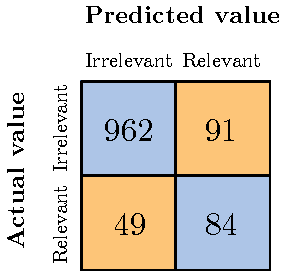
\includegraphics[scale=1]{figures/conf_matrices/ita_rel_logreg/ita_rel_logreg_bfs.pdf}
	\label{fig:ita_rel_logreg_bfs}
\end{figure}

\begin{center}
	\begin{tabular}{ | c | c | } 
		\hline
		\textbf{F1-macro} & 0.545 \\
		\hline
		\textbf{Recall} & 0.631 \\ 
		\hline
		\textbf{Precision} & 0.480 \\ 
		\hline
	\end{tabular}
\end{center}

Features' selection has been made exploiting L1-regularization on model training. The effect is shown in Figure \ref{fig:ita_rel_logreg_fs}, where it is possible to verify the early discussed characteristic: L1-regularization selects almost automatically most important features nullifying less important ones. Setting the cutoff value to 0.1, the method returns 1349 final values.\\

% fs
\begin{figure}[H]
	\centering
	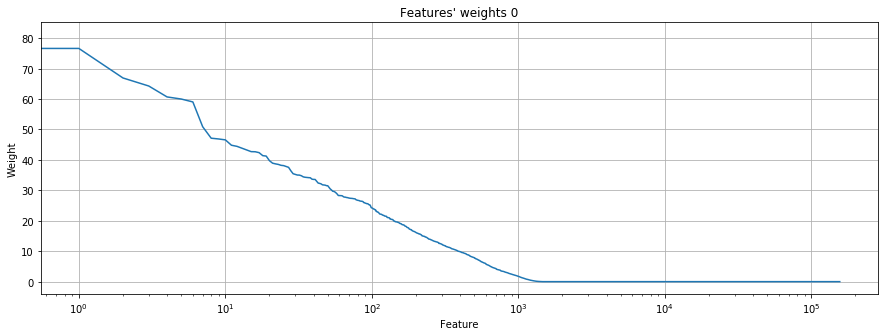
\includegraphics[width=\textwidth]{figures/conf_matrices/ita_rel_logreg/ita_rel_logreg_fs.png}
	\caption{Features' weights of Logistic Regression classifier for relevance detection before features selection}
	\label{fig:ita_rel_logreg_fs}
\end{figure}

After features selection the scores, obtained with the model with $C$=1000, become:

% LR fs
\begin{figure}[H]
	\centering
	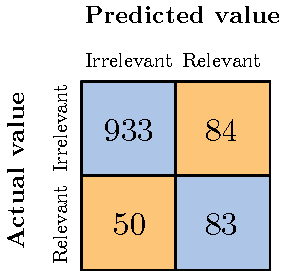
\includegraphics[scale=1]{figures/conf_matrices/ita_rel_logreg/ita_rel_logreg_afs.pdf}
	\label{fig:ita_rel_logreg_afs}
\end{figure}

% LR after fs
\begin{center}
	\begin{tabular}{ | c | c | } 
		\hline
		\textbf{F1-macro} & 0.553 \\
		\hline
		\textbf{Recall} & 0.624 \\ 
		\hline
		\textbf{Precision} & 0.497 \\ 
		\hline
	\end{tabular}
\end{center}

% TODO most important features
\textcolor{red}{MOST IMPORTANT FEATURES}

From the confusion matrix it is possible to notice that the features selection improves mostly the precision, in fact it reduces the number of true positives from 91 to 84, while the recall remains similar.\\
Comparing the results with the SVM classifier, both reach similar results for what concerns the F1-macro score, but the Logistic Regression one gets a better recall, that makes it the preferable one.



\subsection{Sentiment Classification with SVM}

For sentiment classification it has been followed an approach similar to the one used for relevance detection: the same preprocessing and vectorization techniques have been applied, so the same is the dimension of the features space. The only thing that has been changed was the classifier, that became multiclass instead of binary. \\
A first result on validation data, obtained with the hyperparameter $C$=10, gave the following scores:

% SVM no fs
\begin{figure}[H]
	\centering
	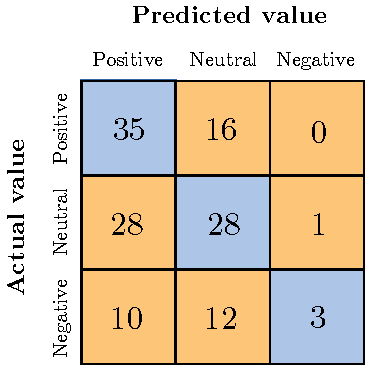
\includegraphics[scale=1]{figures/conf_matrices/ita_snt_svm/ita_snt_svm_bfs.pdf}
	\label{fig:ita_snt_svm_bfs}
\end{figure}

\begin{center}
	\begin{tabular}{ | c | c | } 
		\hline
		\textbf{F1-macro} & 0.422 \\
		\hline
		\textbf{F1-micro} & 0.496 \\ 
		\hline
	\end{tabular}
\end{center}

% fs
For simplicity in Figure \ref{fig:ita_snt_svm_fs} it has been shown just one of the three classifiers' weights that compose the one-versus-one multiclass classifier for sentiment classification. All graphics actually have the same shape, which is typical. Setting the cutoff values, respectively to 0.15, 0.1 and 0.1, the number of selected features become 9657, which is again much lower than initial dimension.

\begin{figure}[H]
	\centering
	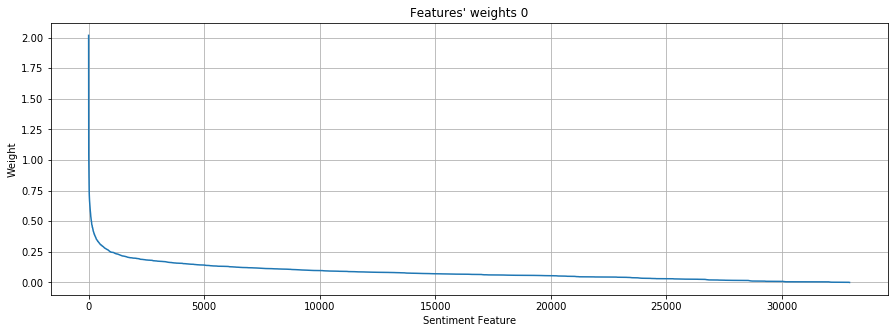
\includegraphics[width=\textwidth]{figures/conf_matrices/ita_snt_svm/ita_snt_svm_fs.png}
	\caption{Features' weights of SVM classifier for sentiment classification before features selection}
	\label{fig:ita_snt_svm_fs}
\end{figure}

% SVM fs
After features selection, the optimized model with $C$=10, the scores become:
\begin{figure}[H]
	\centering
	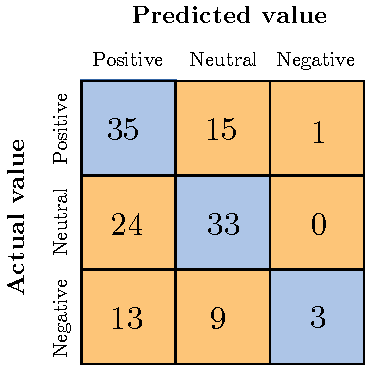
\includegraphics[scale=1]{figures/conf_matrices/ita_snt_svm/ita_snt_svm_afs.pdf}
	\label{fig:ita_snt_svm_afs}
\end{figure}

\begin{center}
	\begin{tabular}{ | c | c | } 
		\hline
		\textbf{F1-macro} & 0.451 \\
		\hline
		\textbf{F1-micro} & 0.534 \\ 
		\hline
	\end{tabular}
\end{center}

The scores notify a little improvement on the performance, that is easily seen in the classification of neutral class. Again, the scores are very different from the one seen for the Twitter's dataset, and the motivation have been already presented. Moreover, for this classification, the bias inducted for the negative class imbalance is visible on the confusion matrix: while positive and neutral classes perform quite well, for what concerns the negative class, the classifier tends to predict positive or neutral. This issue will be present in all other models, and it is characteristics the fact that the dataset is unbalanced.\\
This model has been used as baseline, in order to compare the effectiveness of the revised BPEF model, which results will be presented in the following paragraph.

\subsection{Sentiment Classification with Revised BPEF}

% BPEF no fs
\begin{figure}[H]
	\centering
	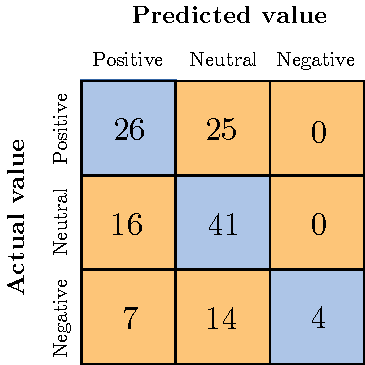
\includegraphics[scale=1]{figures/conf_matrices/ita_snt_bpef/ita_snt_bpef_bfs.pdf}
	\label{fig:ita_snt_bpef_bfs}
\end{figure}

\begin{center}
	\begin{tabular}{ | c | c | } 
		\hline
		\textbf{F1-macro} & 0.465 \\
		\hline
		\textbf{F1-micro} & 0.534 \\ 
		\hline
	\end{tabular}
\end{center}

% fs

% BPEF fs
\begin{figure}[H]
	\centering
	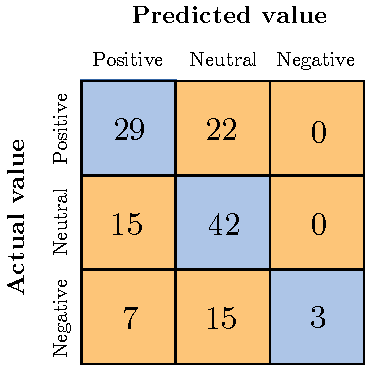
\includegraphics[scale=1]{figures/conf_matrices/ita_snt_bpef/ita_snt_bpef_afs.pdf}
	\label{fig:ita_snt_bpef_afs}
\end{figure}

\begin{center}
	\begin{tabular}{ | c | c | } 
		\hline
		\textbf{F1-macro} & 0.467 \\
		\hline
		\textbf{F1-micro} & 0.556 \\ 
		\hline
	\end{tabular}
\end{center}

\subsection{4-labels Classification with SVM}

% 4 labels SVM bfs
\begin{figure}[H]
	\centering
	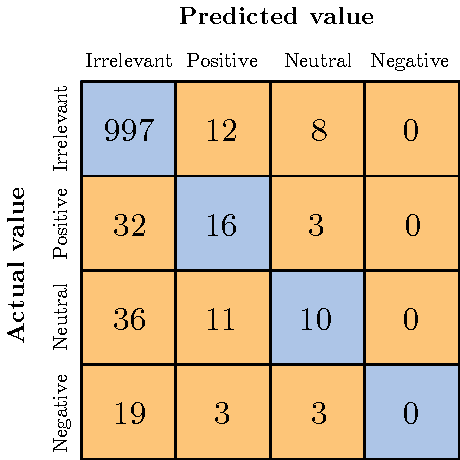
\includegraphics[scale=1]{figures/conf_matrices/ita_4l_svm/ita_4l_svm_bfs.pdf}
	\label{fig:ita_4l_svm_bfs}
\end{figure}

\begin{center}
	\begin{tabular}{ | c | c | } 
		\hline
		\textbf{F1-macro} & 0.385 \\
		\hline
		\textbf{F1-micro} & 0.890 \\ 
		\hline
	\end{tabular}
\end{center}

% fs
% TODO fs


% 4 labels SVM afs
\begin{figure}[H]
	\centering
	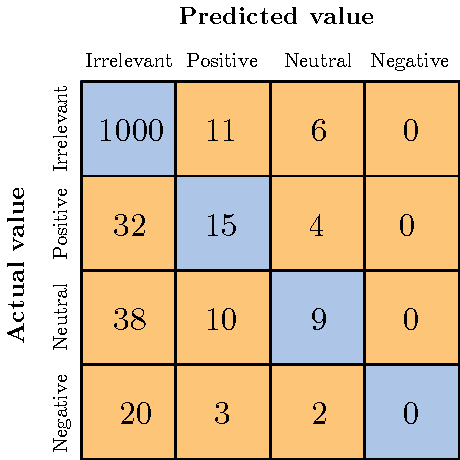
\includegraphics[scale=1]{figures/conf_matrices/ita_4l_svm/ita_4l_svm_afs.pdf}
	\label{fig:ita_4l_svm_afs}
\end{figure}

\begin{center}
	\begin{tabular}{ | c | c | } 
		\hline
		\textbf{F1-macro} & 0.378 \\
		\hline
		\textbf{F1-micro} & 0.890 \\ 
		\hline
	\end{tabular}
\end{center}


\subsection{4-labels Classification with Cascade Classifier}

% cascade SVM val
\begin{figure}[H]
	\centering
	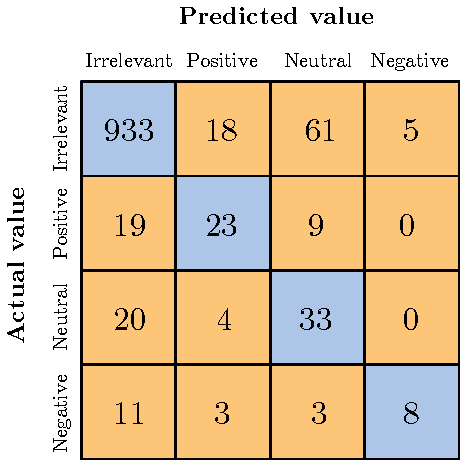
\includegraphics[scale=1]{figures/conf_matrices/ita_cascade_bpef/ita_cascade_bpef_val.pdf}
	\label{fig:ita_cascade_svm_val}
\end{figure}

\begin{center}
	\begin{tabular}{ | c | c | } 
		\hline
		\textbf{F1-macro} & 0.378 \\
		\hline
		\textbf{F1-micro} & 0.890 \\ 
		\hline
	\end{tabular}
\end{center}


% cascade BPEF val
\begin{figure}[H]
	\centering
	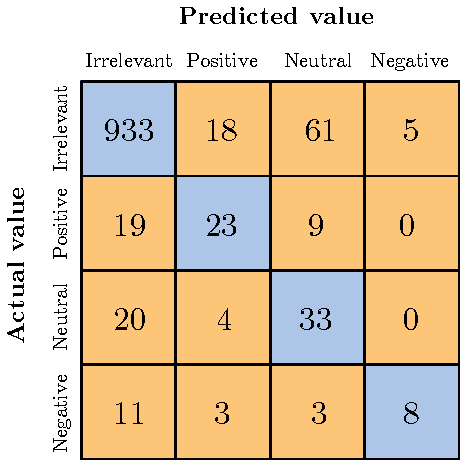
\includegraphics[scale=1]{figures/conf_matrices/ita_cascade_bpef/ita_cascade_bpef_val.pdf}
	\label{fig:ita_cascade_bpef_val}
\end{figure}

\begin{center}
	\begin{tabular}{ | c | c | } 
		\hline
		\textbf{F1-macro} & 0.378 \\
		\hline
		\textbf{F1-micro} & 0.890 \\ 
		\hline
	\end{tabular}
\end{center}




\subsection{4-labels Classification with Test Data}

% cascade SVM test
\begin{figure}[H]
	\centering
	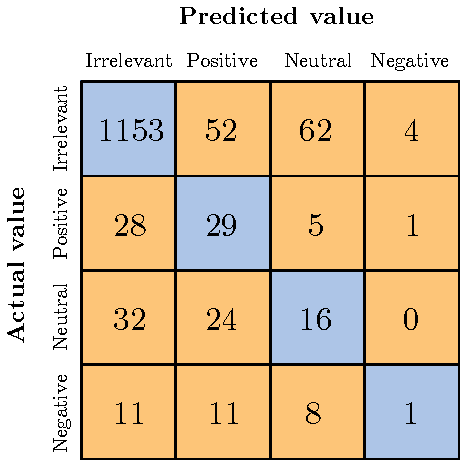
\includegraphics[scale=1]{figures/conf_matrices/ita_cascade_svm/ita_cascade_svm_tst.pdf}
	\label{fig:ita_cascade_svm_tst}
\end{figure}

\begin{center}
	\begin{tabular}{ | c | c | } 
		\hline
		\textbf{F1-macro} & 0.375 \\
		\hline
		\textbf{F1-micro} & 0.834 \\ 
		\hline
	\end{tabular}
\end{center}


% cascade BPEF test
\begin{figure}[H]
	\centering
	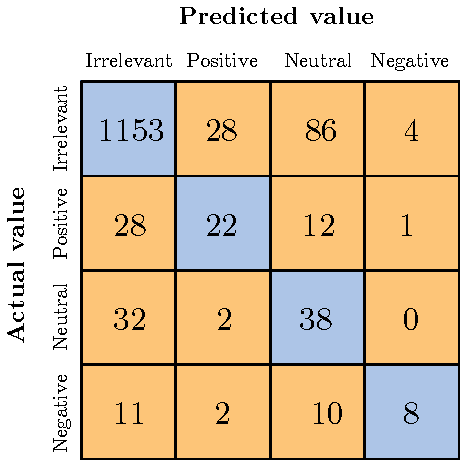
\includegraphics[scale=1]{figures/conf_matrices/ita_cascade_bpef/ita_cascade_bpef_tst.pdf}
	\label{fig:ita_cascade_bpef_tst}
\end{figure}

\begin{center}
	\begin{tabular}{ | c | c | } 
		\hline
		\textbf{F1-macro} & 0.503 \\
		\hline
		\textbf{F1-micro} & 0.850 \\ 
		\hline
	\end{tabular}
\end{center}



\subsection{Classification with other Classes}


\section{Data Visualization}